\documentclass[11pt, a4paper]{article}
\usepackage[utf8]{inputenc}
\usepackage{amsmath,setspace,geometry}
\usepackage{amsthm}
\usepackage{amsfonts}
\usepackage{mathtools}
\mathtoolsset{showonlyrefs}
\usepackage[shortlabels]{enumitem}
\usepackage{rotating}
\usepackage{pdflscape}
\usepackage{graphicx}
\usepackage{bbm}
\usepackage[dvipsnames]{xcolor}
\usepackage[colorlinks=true, linkcolor= RawSienna, citecolor = RawSienna, filecolor = RawSienna, urlcolor = RawSienna, hypertexnames = true, backref = page]{hyperref}
\usepackage[]{natbib} 
\bibpunct[:]{(}{)}{,}{a}{}{,}
\geometry{left = 1.0in,right = 1.0in,top = 1.0in,bottom = 1.0in}
\usepackage[english]{babel}
\usepackage{float}
\usepackage{caption}
\usepackage{subcaption}
\usepackage{tikz}
\usepackage{booktabs}
\usepackage{pdfpages}
\usepackage{threeparttable}
\usepackage{framed}
\usepackage{comment}
\usepackage{lscape}
\usepackage{bm}
\setstretch{1.3}
%\usepackage[tablesfirst,nolists]{endfloat}

\usepackage[T1]{fontenc}
\usepackage{mlmodern}  % 太いComputer Modern
% MLmodernのバグを修正: cf. https://tex.stackexchange.com/questions/646333/size-of-integral-symbol-in-section-header-with-mlmodern
\DeclareFontFamily{OMX}{mlmex}{}
\DeclareFontShape{OMX}{mlmex}{m}{n}{<->mlmex10}{} 
\usepackage{tgtermes} % 数式以外の欧文をTXフォントで上書き

\newtheorem{theorem}{Theorem}
\newtheorem{assumption}{Assumption}
\newtheorem{lemma}{Lemma}
\newtheorem{definition}{Definition}
\newtheorem{proposition}{Proposition}
\newtheorem{claim}{Claim}
\newtheorem{corollary}{Corollary}
\newtheorem{example}{Example}
\DeclareMathOperator{\rank}{rank}

\theoremstyle{remark}
\newtheorem{remark}{Remark}

\title{Note on Lau (1982)}
\author{Yuri Matsumura\thanks{\href{mailto:}{yuri.matsumura23@gmail.com}, Department of Economics, Rice University.} \and Suguru Otani \thanks{\href{mailto:}{suguru.otani@e.u-tokyo.ac.jp}, Market Design Center, Department of Economics, University of Tokyo
\\Declarations of interest: none %this is for Economics Letters
}}

\begin{document}

\maketitle
\begin{abstract}
    TBA
\end{abstract}

\noindent\textbf{Keywords:} Conduct parameters, Homogenous Goods Market, Mathematical Programming with Equilibrium Constraints, Monte Carlo simulation
\vspace{0in}
\newline
\noindent\textbf{JEL Codes:} C5, C13, L1

\bigskip

\section{Model}
Consider a homogeneous product market where a representative firm maximizes its profit, given by the function\footnote{See \citet{adachiMicrofoundation2023} for the detail of the interpretation.}:
\begin{align}
    \Pi = P(Q)Q - C(Q),
\end{align}
where $P(Q)$ represents the aggregate inverse demand function, and $C(Q$ is the aggregate cost function.
Assume that the demand function is decreasing in $Q$, $P'(Q) \equiv \frac{dP}{dQ} < 0$ and the cost function is increasing in $Q$, $C'(Q) \equiv \frac{dC}{dQ} > 0$.

To determine the optimal quantity (or equilibrium quantity), the firm adjusts the quantity such that the marginal gain from increasing the quantity equals the marginal loss. 
However, the firm recognizes only a fraction of the marginal gain, denoted by $\theta \in [0,1]$. 
As a result, the equilibrium condition can be written as:
\begin{align}
    \theta P'(Q)Q = - (P(Q) - C'(Q)),
\end{align}
where $C'(Q)$ represents the marginal cost of production.
The left hand is the marginal gain by increasing price and the right hand represents the marginal loss.
By rewriting the relationship, we have
\begin{align}
    p + \theta P'(Q)Q = C'(Q). \label{eq:optimality_conditition}
\end{align}
This relationship is easy to interpret when $\theta = 1$ because it corresponds to the first-order condition of a monopoly firm.
Additionally, depending on the value of $\theta$, the formula can nest the first-order condition of other models such as perfect competition ($\theta=0$) and Cournot competition ($\theta=1/N$) 

\cite{bresnahan1982oligopoly} considers the identification of $\theta$ in linear demand and linear marginal cost model, and \citet{lau1982identifying} attempts to simultaneously identify both the conduct parameter and the marginal cost function in a more general setting.
Define the aggregate inverse demand and aggregate marginal cost function as
\begin{align}
    p = P(Q, X^{d}),\text{ and } \quad mc = MC(Q, X^{s}),
\end{align}
where $Q$ is the aggregate quantity, $X^{d}$ and $X^{s}$ are the vector of exogenous variables.
Assume that $X^{d}$ and $X^{s}$ are exclusive, that is, there is no common variable in $X^{d}$ and $X^{s}$.
In this sense, $X^{d}$ works as demand shifters and $X^{s}$ works as cost shifters. 
Then, \eqref{eq:optimality_conditition} becomes
\begin{align}
     P(Q,X^{d}) + \theta\frac{\partial P}{\partial Q}(Q, X^{d})Q = MC(Q, X^{s}),\label{eq:supply_equation}
\end{align}
\eqref{eq:supply_equation} is referred as "supply equation" in \citet{bresnahan1982oligopoly}.
Note that as $X^{s}$ works as exclusive cost shifter, we can assume that the demand function is identified.
Then, \citet{lau1982identifying} considers the identification of the conduct parameter and the marginal cost function. 
Instead of directly proving identification, \citet{lau1982identifying} takes an indirect approach by specifying the conditions under which the model is not identified. 
The definition of non-identification in this model is as follows:

\begin{framed}
    \begin{definition}\label{def:non_identification}
    Non-identification implies for any $X^{d}$ and $X^{s}$,
    \begin{align}
    P(Q, X^{d}) + \theta \frac{\partial P}{\partial Q}(Q, X^{d})Q &= MC(Q, X^{s}),  \label{eq:foc_alpha}\\
    P(Q, X^{d}) + \theta^{*} \frac{\partial P}{\partial Q}(Q, X^{d})Q &= MC^{*}(Q, X^{s}),\label{eq:foc_beta}
    \end{align}
    where $\theta \neq \theta^{*}$, $g \ne g'$,\footnote{This condition is not stated in \citet{lau1982identifying}, but assuming $g = g'$ makes the identification simple.} and the reduced form functions $Q = h(X^{d}, X^{s})$ and $Q = h^{*}(X^{d}, X^{s})$ defined by \eqref{eq:foc_alpha} and \eqref{eq:foc_beta} respectively are identical.
    \end{definition}
\end{framed}
In other words, non-identification asks the following question: given an identified inverse demand function $P$, is it possible to find two distinct pairs of conduct parameter and marginal cost, $\Lambda = (\theta, MC)$ and $\Lambda^{*} = (\theta^{*}, MC^{*})$, that lead to observable equivalent equilibrium?

\citet{lau1982identifying} presents the condition on the demand function under which the conduct parameter cannot be identified:
\begin{framed}
\begin{theorem}\label{theorem_lau}
    Under the assumption that the industry inverse demand and cost functions are twice continuously differentiable, the index of competitiveness $\theta$ cannot be identified from data on industry price and output and other exogenous variables alone if and only if the industry inverse demand function is separable in $X^{d}$, that is,
    \begin{align}
        p = P(Q, r(X^{d})), \label{eq:demand_separable}
    \end{align}
    but not take the form, 
    \begin{align}
        P = Q^{-1/\theta}r(X^{d}) + s(Q). \label{eq:identification_separable}
    \end{align}
\end{theorem}
\end{framed}
The theorem implies that the conduct parameter is identified when the demand function is not separable, except \eqref{eq:identification_separable}.

\begin{comment}
    \citet{bresnahan1982oligopoly} considers a model with linear demand and marginal cost.
    He considers a demand function such that $P = \alpha_0 + (\alpha_1 + \alpha_2 Z) Q + \alpha_3 Y + \alpha_4 Z  + \varepsilon$ where $Z$ is called a demand rotation instrument.
    It is easy to verify that this demand is not separable.
    Under the demand, the conduct parameter and the marginal cost parameter can be identified.
    \citet{matsumura2023resolving} provide more detailed conditions for the identification.
\end{comment}


\section{Summary of Goldman and Uzawa (1964)}
Before investigating the proof of Lau, we introduce results in \citet{goldmanNote1964}, which Lau also relies on.
\citet{goldmanNote1964} consider the following setting.
Let $n$ be the number of variables and $x = (x_{1},\ldots, x_{n})$ be a vector of $n$ variables.
Consider a partition of $X$ into $K$ parts, $\{x^1, \ldots, x^K\}$ such that $X = \bigcup_{k=1}^K x^k$ and $x^k \cap x^l = \emptyset$ for $k\ne l$.
\begin{framed}
    \begin{definition}\label{def:weal_separable}
        A function is weakly separable with respect to the partition if 
        \begin{align}
            \frac{\partial}{\partial x_l}\left(\frac{\partial f/\partial x_i}{\partial f/\partial x_j}\right) = 0, \quad i,j\in x^k, l \notin x^k.
        \end{align}
    \end{definition}
\end{framed}
This implies that the ratio of the derivative with respect to $x_i$ and $x_j$, which are in the same category, is not affected by the change in the variables in other partitions.
Intuitively, by taking the ratio, the component of $f$ relating to $x_l$ is canceled out, and hence the derivative of the ratio with respect to $x_l$ becomes zero.
When $f$ is a utility function, this implies that the marginal rate of substitution between commodity $i$ and $j$ in the same partition is independent of the quantities of commodities outside $x^k$.

Then, \citet{goldmanNote1964} specifies the functional form that a weak separable function should satisfy.
\begin{framed}
    \begin{theorem}\label{thorem_2_GU}
    A function $f(x)$ is weakly separable with respect to a partition $\{x^1, .. ., x^K\}$ if and only if $f(x)$ is of the form: 
    \begin{align}
        f(X) = \Phi(r^1(x^{1}),\ldots, r^K(x^{K})   )
    \end{align} where $\Phi(r^1,\ldots, r^K)$ is a function of $K$ variables and, for each $k$, $r^k(x^{k})$ is a function subvector $x^{k}$ alone.
    \end{theorem}
\end{framed}


Let $\{Q,X_{1}^{d}, \ldots,  X_{K_d}^{d}\}$ be a vector of variables where $K_d$ is the dimension of $X^{d}$.
Consider a partition $\{Q, X^{d}\}$, and let $r^1(Q) = Q$.
Then, $P(Q, r(X^{d}))$ satisfies the form in Theorem \ref{thorem_2_GU}.
Therefore, the definition of separable function in Theorem \ref{theorem_lau} corresponds to the functional form in  Theorem \ref{thorem_2_GU}, which implies that the separability in \citet{lau1982identifying} corresponds to the weak separability in \citet{goldmanNote1964}.
By Definition \ref{def:weal_separable}, the separable function \eqref{eq:demand_separable} should satisfy
\begin{align}
    \frac{\partial }{\partial Q} \left(\frac{\partial P/\partial X_{i}^{d}}{\partial P/\partial X_{j}^{d}} \right) = 0,\quad i \ne j, 
\end{align}
where $X_{i}^{d}$ is the $i$-th element in $X^{d}$.

\begin{remark}
    The linear demand function in \citet{bresnahan1982oligopoly} is not separable:
    \begin{align}
        \frac{f_Z}{f_Y} = \frac{\alpha_2 Q}{\alpha_3} \Longrightarrow \frac{\partial P_Z/f_Y}{\partial Q} = \frac{\alpha_2}{\alpha_3} \ne 0,
    \end{align}
    where $\alpha_2/\alpha_3 \ne 0$ comes from the sufficient condition for the identification in \citet{matsumura2023resolving}.
    Thus the conduct parameter can be identified.
    \qed
\end{remark}



\begin{framed}
\begin{lemma}\label{lemma_1_GU}
    Let $f(x)$ and $g(x)$ be two continuously twice-differentiable functions of $n$ variables $x=(x_1, \dots, x_n)$. If each indifference surface is connected, and if there exists a function $\lambda(x)$ such that
    \begin{align}
    f_i(x) &= \lambda(x)g_i(x), \quad i=1, \dots, n, \quad \text{for all } x, \label{eq:transform_f}
    \end{align}
    then $f(x)$ is a transformation of $g(x)$; namely, there exists a function $T(\cdot)$ of one variable such that
    \begin{align}
    f(x) &= T(g(x)) \quad \text{for all } x.
    \end{align}
    Hence, in particular, the function $\lambda(x)$ satisfying \eqref{eq:transform_f} must be of the form:
    \begin{align}
        \lambda(x) &= \Lambda(g(x)) \quad \text{for all } x, \label{eq:form_of_lambda}
    \end{align}
    with some function $\Lambda(\cdot)$ of one variable.
\end{lemma}
\end{framed}


\section{Proof in Lau(1982)}\label{sec:proof_lau}
Now, let's investigate the proof of \citet{lau1982identifying}.
We try to fill some gaps between the lines in the original proof.






% Proof of necessity
\subsection{Necessity: non-identification implies that the demand function is separable}

Suppose that $(\theta, MC)$ is the pair of the true model component, but there is another pair $(\theta^{*}, MC^{*})$ that leads to an observable equivalent equilibrium.
Given $X^{d}$ and $X^{s}$, the true component $(\theta, MC)$ satisfy the first-order condition for quantity $Q$,
\begin{align}
    F(Q, X^{d}, X^{s}) \equiv P(Q, X^{d}) + \theta\frac{\partial P}{\partial Q}(Q, X^{d})Q - MC(Q, X^{s}) = 0.
\end{align}
Assume that we can solve the first-order condition and obtain the reduced-form equation for the equilibrium quantity, $Q^e$.
Assume that the derivative of $F$ with respect to $Q$ at the equilibrium quantity $Q^e$ is nonzero;
\begin{align}
    \frac{\partial F}{\partial Q}(Q^e, X^{d}, X^{s}) = (1+\theta)\frac{\partial P}{\partial Q}(Q^e, X^{d}) + \theta\frac{\partial^2 P}{\partial Q^2}(Q^e, X^{d})Q^e - \frac{\partial MC}{\partial Q}(Q^e, X^{s}) \ne 0.
\end{align}
Then, we can apply the implicit function theorem, and hence, the equilibrium quantity has a reduced-form equation $Q^e = h(X^{d}, X^{s})$.
The derivatives of $F$ for each variable are
\begin{align}
    \frac{\partial F}{\partial X^{d}_i}(Q^e, X^{d}, X^{s}) & =  \frac{\partial P}{\partial X^{d}_{i}}(Q^e, X^{d}) + \theta\frac{\partial^2 P}{\partial X^{d}_{i}\partial Q}(Q^e, X^{d})Q^e,\\
    \frac{\partial F}{\partial X^{s}_i}(Q^e, X^{d}, X^{s}) & =  -\frac{\partial MC}{\partial X^{s}_{i}}(Q^e, X^{s}),\\
    \frac{\partial F}{\partial Q}(Q^e, X^{d}, X^{s}) & = (1+\theta)\frac{\partial P}{\partial Q}(Q^e, X^{d}) + \theta\frac{\partial^2 P}{\partial Q^2}(Q^e, X^{d})Q^e - \frac{\partial MC}{\partial Q}(Q^e, X^{s}).
\end{align}
Then, the implicit function theorem implies that the derivative of $h$ with respect to the demand shifter and the cost shifters are
\begin{align}
    \frac{\partial h}{\partial X^{d}_{i}}(X^{d}, X^{s}) = -\frac{\frac{\partial P}{\partial X^{d}_{i}}(Q^e, X^{d}) + \theta\frac{\partial^2 P}{\partial X^{d}_{i}\partial Q}(Q^e, X^{d})Q^e }{(1+\theta)\frac{\partial P}{\partial Q}(Q^e, X^{d}) + \theta\frac{\partial^2 P}{\partial Q^2}(Q^e, X^{d})Q^e - \frac{\partial MC}{\partial Q}(Q^e, X^{s})}, \label{eq:foc_derivative_demand}
\end{align}
and
\begin{align}
    \frac{\partial h}{\partial X^{s}_{i}}(X^{d}, X^{s}) & = \frac{\frac{\partial MC}{\partial X^{s}_{i}}(Q^e, X^{s})}{(1+\theta)\frac{\partial P}{\partial Q}(Q^e, X^{d}) + \theta\frac{\partial^2 P}{\partial Q^2}(Q^e, X^{d})Q^e - \frac{\partial MC}{\partial Q}(Q^e, X^{s})}. \label{eq:foc_derivative_supply}
\end{align}


% Apply the implicit function theorem to h^*
By applying the same argument for \eqref{eq:foc_beta}, we obtain 
\begin{align}
    \frac{\partial h^{*}}{\partial X^{d}_{i}}(X^{d}, X^{s}) &= -\frac{\frac{\partial P}{\partial X^{d}_{i}}(Q^e, X^{d}) + \theta^{*}\frac{\partial^2 P}{\partial X^{d}_{i}\partial Q}(Q^e, X^{d})Q^e }{(1+\theta^{*})\frac{\partial P}{\partial Q}(Q^e, X^{d}) + \theta^{*}\frac{\partial^2 P}{\partial Q^2}(Q^e, X^{d})Q^e - \frac{\partial MC^{*}}{\partial Q}(Q^e, X^{s})}, \\
    \frac{\partial h^{*}}{\partial X^{s}_{i}}(X^{d}, X^{s}) & = \frac{\frac{\partial MC^{*}}{\partial X^{s}_{i}}(Q^e, X^{s})}{(1+\theta^{*})\frac{\partial P}{\partial Q}(Q^e, X^{d}) + \theta^{*}\frac{\partial^2 P}{\partial Q^2}(Q^e, X^{d})Q^e - \frac{\partial MC^{*}}{\partial Q}(Q^e, X^{s})}.
\end{align}

 
% Use the definition of non-identification
Hereafter, for notational simplicity, I suppress $(Q^e, X^{d}, X^{s})$.
As the non-identification implies that $Q^e = h(X^{d}, X^{s}) = h^{*}(X^{d}, X^{s})$ for all $X^{d}$ and $X^{s}$, we have
\begin{align}
    \frac{\partial h^{*}}{\partial X^{d}_{i}}(X^{d}, X^{s})  = \frac{\partial h}{\partial X^{d}_{i}}(X^{d}, X^{s})\quad \text{  and  } \quad \frac{\partial h^{*}}{\partial X^{s}_{i}}(X^{d}, X^{s})  = \frac{\partial h}{\partial X^{s}_{i}}(X^{d}, X^{s}) . \label{eq:observale_equivalence_derivative}
\end{align}
Thus, we obtain 
\begin{align}
     \frac{\partial h^{*}}{\partial X^{d}_{i}}  = - \frac{\frac{\partial P}{\partial X^{d}_{i}} + \theta^{*}\frac{\partial^2 P}{\partial X^{d}_{i}\partial Q}Q^e }{(1+\theta^{*})\frac{\partial P}{\partial Q} + \theta^{*}\frac{\partial^2 P}{\partial Q^2}Q^e - \frac{\partial MC^{*}}{\partial Q^e}} = - \frac{\frac{\partial P}{\partial X^{d}_{i}} + \theta \frac{\partial^2 P}{\partial X^{d}_{i}\partial Q}Q^e }{(1+\theta)\frac{\partial P}{\partial Q} + \theta\frac{\partial^2 P}{\partial Q^2}Q^e - \frac{\partial MC}{\partial Q}} =  \frac{\partial h}{\partial X^{d}_{i}} \label{eq:derivative_q_x_d}
\end{align}
and
\begin{align}
     \frac{\partial h^{*}}{\partial X^{s}_{i}} = \frac{\frac{\partial MC^{*}}{\partial X^{s}_{i}}}{(1+\theta^{*})\frac{\partial P}{\partial Q} + \theta^{*}\frac{\partial^2 P}{\partial Q^2}Q^e - \frac{\partial MC^{*}}{\partial Q}} & = \frac{\frac{\partial MC}{\partial X^{s}_{i}}}{(1+\theta)\frac{\partial P}{\partial Q} + \theta\frac{\partial^2 P}{\partial Q^2}Q^e - \frac{\partial MC}{\partial Q}} =  \frac{\partial h}{\partial X^{s}_{i}} .\label{eq:derivative_q_x_s}
\end{align}

% Define the lambda function
Note that the denominators in \eqref{eq:derivative_q_x_d} and \eqref{eq:derivative_q_x_s} are nonzero.
Hence, we can define $\lambda(X^{d}, X^{s})$ such that
\begin{align}
    \lambda( X^{d}, X^{s}) \equiv \frac{(1+\theta^{*})\frac{\partial P}{\partial Q}(Q^e, X^{d}) + \theta^{*}\frac{\partial^2 P}{\partial Q^2}(Q^e, X^{d})Q^e - \frac{\partial MC^{*}}{\partial Q}(Q^e, X^{s})}{(1+\theta)\frac{\partial P}{\partial Q}(Q^e, X^{d}) + \theta\frac{\partial^2 P}{\partial Q^2}(Q^e, X^{d})Q^e - \frac{\partial MC}{\partial Q}(Q^e, X^{s})}.\label{eq:lambda_q_x}
\end{align}
Lau defines $\lambda$ function as the function of $Q$ and $X^{d}$ or $X^{s}$ and apply only for  \eqref{eq:derivative_q_x_s}.
Here, we explicitly use the fact that the quantity is fixed at $Q^e$; thus, the right-hand side of \eqref{eq:lambda_q_x} is a function of $X^{d}$ and $X^{s}$, and hence $\lambda$ is defined as the function of 
$X^{d}$ and $X^{s}$.

% 均衡数量周りでのhの変化が同じになる.
%もし陰関数定理を適応するのであれば,hの微分は均衡数量周りでしか成立しないはず.
%その点で,Tによる変換も実際はQが取りうるすべての値で成立するわけではなくて,均衡数量周りでしか成立しないと考える方がただしいのか?




% Non-identification implies that there is a transformation for the inverse demand and the marginal cost 
Then, \eqref{eq:derivative_q_x_d} and \eqref{eq:derivative_q_x_s} implies that 
\begin{align}
    &\frac{\partial P}{\partial X^{d}_{i}}(Q^e, X^{d}) + \theta^{*}\frac{\partial^2 P}{\partial X^{d}_{i}\partial Q}(Q^e, X^{d})Q^e \\
    &\hspace{2cm} = \lambda(X^{d}, X^{s})\left[\frac{\partial P}{\partial X^{d}_{i}} (Q^e, X^{d})+ \theta \frac{\partial^2 P}{\partial X^{d}_{i}\partial Q}(Q^e, X^{d})Q^e\right],\label{eq:transform_demand}
\end{align}
and
\begin{align}
    \frac{\partial MC^{*}}{\partial X^{s}_{i}}(Q^e, X^{s}) & = \lambda(X^{d}, X^{s})\frac{\partial MC}{\partial X^{s}_{i}}(Q^e, X^{s}).\label{eq:transform_mc}
\end{align}
By applying Lemma \ref{lemma_1_GU} to \eqref{eq:transform_demand} and \eqref{eq:transform_mc}, there exist a $T$ such that
\begin{align}
    P(Q^e, X^{d}) + \theta^{*} \frac{\partial P}{\partial Q}(Q^e, X^{d}) Q^e & = T\left(P(Q^e, X^{d}) + \theta \frac{\partial P}{\partial Q}(Q^e, X^{d}) Q^e\right) \label{eq:transformation_T_demand}
\end{align}
and
\begin{align}
    MC^{*}(Q^e, X^{s}) = T(MC(Q^e, X^{s})). \label{eq:transformation_T_mc}
\end{align}
Therefore, the first-order condition under the true component $(\theta, MC)$ can be transformed into the first-order condition under $(\theta^*, MC^*)$ through $T$ while keeping the equilibrium quantity the same.

In other words, given $(\theta, MC)$ and $\theta^{*}$, $T$ can generate an observable equivalent equilibrium.
Under the true component $(\theta, MC)$, we can obtain the equilibrium quantity $Q^{e}$.
This quantity should solve the first-order condition 
\begin{align}
    P(Q^e, X^d) + \theta \frac{\partial P}{\partial Q}(Q^e, X^d) Q^e = MC(Q^e, X^{s}).
\end{align}
Then, by applying $T$, we have
\begin{align}
    P(Q^e, X^d) + \theta^{*} \frac{\partial P}{\partial Q}(Q^e, X^d) Q^e 
    & = T\left(P(Q^e, X^d) + \theta \frac{\partial P}{\partial Q}(Q^e, X^d) Q^e\right) \\
    &= T( MC(Q^e, X^{s})).
\end{align}
Define $MC^{*}(Q, X^{s}) \equiv T(MC(Q, X^{s}))$.
Then, the above relationship implies that $Q^{e}$ also solves the first-order condition under $(\theta^{*}, MC^{*})$;
\begin{align}
    P(Q^e, X^d) + \theta^{*} \frac{\partial P}{\partial Q}(Q^e, X^d) Q^e = MC^{*}(Q^e, X^{s}).
\end{align}
Therefore, two distinct pairs of the conduct parameter and the marginal cost lead to the same equilibrium quantity.

\textcolor{red}{An important note is this relationship holds only at the equilibrium quantity. 
In this sense, when $X^{d}$ or $X^{s}$ move, $Q^e$ also moves. 
Thus, the transformation does not necessarily hold for any combination of $Q, X^{d}$ and $X^{s}$.}







\subsubsection{The cases where observable equivalence does not hold}
% Additional argument for there is the transformation T.
So far, we have not imposed any restriction on the inverse demand and the marginal cost except for twice-continuous differentiability.
However, we should impose additional restrictions to apply Lemma \ref{lemma_1_GU} because, depending on the functional form, there are cases where observable equivalence is violated.
In other words, the relation in \eqref{eq:derivative_q_x_d} and \eqref{eq:derivative_q_x_s} do not hold depending on the functional form of $P$ and $MC$.

% Lau 自身の議論

\begin{remark}
Lau relates this argument with the singularity of the transformation $T$.
First, Lau only derives \eqref{eq:transform_mc} and \eqref{eq:transformation_T_mc}.
Then, substitute the left-hand side of the first-order condition into \eqref{eq:transformation_T_mc} to get \eqref{eq:transformation_T_demand}.
By differentiate \eqref{eq:transformation_T_demand} with respect to $X^{d}_i$, obtaining
\begin{align}
\frac{\partial P}{\partial X^{d}_i}(Q, X^{d}) + \theta^{*}\frac{\partial^2 P}{\partial X^{d}_i \partial Q}(Q, X^{d})Q &= T_{1} \cdot \left[\frac{\partial P}{\partial X^{d}_i}(Q, X^{d}) + \theta \frac{\partial^2 P}{\partial X^{d}_i \partial Q}(Q, X^{d})Q\right]\label{eq:transform_theta_derivative_first}
\end{align}
where $T_1$ is the derivative of $T$ with respect to the first element.
Based on this equation, Lau considers when $T$ does not work well as the transformation.
It is obvious that when 
\begin{align}
    \frac{\partial P}{\partial X^{d}_{i}}(Q, X^{d}) + \theta \frac{\partial^2 P}{\partial X^{d}_{i}\partial Q}(Q, X^{d})Q = 0,\\
    \frac{\partial P}{\partial X^{d}_{i}}(Q, X^{d}) + \theta^{*} \frac{\partial^2 P}{\partial X^{d}_{i}\partial Q}(Q, X^{d})Q \ne 0,
\end{align}
the left-hand side of \eqref{eq:transform_theta_derivative_first} is nonzero, but the right-hand side is zero.
Thus, the change in $X_{i}^d$ is not properly transformed from the right-hand side to the left-hand side.
Lau calls this situation "$T$ is singular."
\qed
\end{remark}


% OEとダイレクトにつなげた議論

In the following, we proceed to the argument which has the same implication with Lau but is based on observable equivalence.
First, suppose that
\begin{align}
    \frac{\partial MC}{\partial X_i^{s}}(Q, X^{s}) = 0, \frac{\partial MC^{*}}{\partial X_i^{s}}(Q, X^{s}) \ne 0.
\end{align}
Then, the right-hand side of \eqref{eq:transform_mc} is zero, although its left-hand side is nonzero.
Thus, \eqref{eq:transform_mc} cannot hold.
This situation also implies that the observable equivalence does not hols because $\frac{\partial h^{*}}{\partial X^{s}_{i}}  \ne \frac{\partial h}{\partial X^{s}_{i}}$ in \eqref{eq:derivative_q_x_s}.
Fortunately, Lau assumes that $X^{s}$ is the vector of cost shifter that affects the marginal cost function, and hence, it is natural to assume that for any marginal cost function $MC$, 
\begin{align}
    \frac{\partial MC}{\partial X_i^{s}}(Q, X^{s}) \ne 0.
\end{align}


% There may not be a transformation for the demand function

In contrast, we need more careful consideration for \eqref{eq:transform_demand}.
Suppose that the inverse demand function $P$ satisfies
\begin{align}
    \frac{\partial P}{\partial X^{d}_{i}}(Q, X^{d}) + \theta \frac{\partial^2 P}{\partial X^{d}_{i}\partial Q}(Q, X^{d})Q = 0,\\
    \frac{\partial P}{\partial X^{d}_{i}}(Q, X^{d}) + \theta^{*} \frac{\partial^2 P}{\partial X^{d}_{i}\partial Q}(Q, X^{d})Q \ne 0. 
\end{align}
This situation violates the observable equivalence because $\frac{\partial h^{*}}{\partial X^{d}_{i}}  \ne \frac{\partial h}{\partial X^{d}_{i}} =0$.
Note that the first equation is a partial differential equation.

% Solve the partial differential equation

To solve the equation, assume that the inverse demand function is a separable function such that 
\[P(Q, X^{d}) = g(Q)h(X^{d}) + s(Q).\]
This is more general than a simple separable function  $P(Q, X^{d}) = g(Q)h(X^{d})$, but as we will see, $s(Q)$ does not affect the following step.
By substituting the separable function into the differential equation, we have 
\begin{align}
   0 & =  g(Q) h_i(X^{d}) + \theta g'(Q)h_i(X^{d}) Q\\
   & = h_i(X^{d})( g(Q) + \theta g'(Q)Q).
\end{align}
When $h_i(X^{d}) = 0$, the inverse demand does not react to the change in $X^{d}$, which is unrealistic in this model.
Therefore, we should assume that $h_i(X^{d}) \ne 0$, and hence we have 
\[g(Q) + \thetag'(Q)Q = 0.\]
This equation is an ordinary differential equation of $Q$.
This can be written as
\begin{align}
    \frac{g'(Q)}{g(Q)} &= -\frac{1}{\theta} \frac{1}{Q}
\end{align}
Because the left-hand side is the derivative of $\log g(Q)$ and the right-hand side is also a derivative of $\log Q$, we have
\begin{align}
        \frac{d}{dQ} \log g(Q) &= -\frac{1}{\theta} \frac{d}{dQ} \log Q.
\end{align}
By integrating this over the domain of $Q$, we have
\begin{align}
    \int_{0}^\infty \frac{d}{dQ} \log g(Q) dQ &= -\frac{1}{\theta} \int_{0}^\infty  \frac{d}{dQ} \log Q dQ \\
    \log g(Q) &= -\frac{1}{\theta} \log Q + C\\
    g(Q) &= C Q^{-\frac{1}{\theta}},
\end{align}
where $C$ is the constant of integration.
Substituting this into $f$, we have 
\begin{align}
    P(Q, X^{d}) = C Q^{-\frac{1}{\theta}} h(X^{d}) + s(Q).
\end{align}
Define $r(X^{d}) = Ch(X^{d})$, and then we have
\begin{align}
    P(Q, X^{d}) &= Q^{-\frac{1}{\theta}} r(X^{d}) + s(Q),
\end{align}
which is the same with \eqref{eq:identification_separable}.

% Check if ∂h^*/∂X_i^d ≠ 0 holds
Now, we check whether $\frac{\partial h^{*}}{\partial X_{i}^{d}} \ne 0$ for an alternative conduct parameter $\theta^{*} \ne \theta$.
By substituting the inverse demand function \eqref{eq:identification_separable}, we have
\begin{align}
    \frac{\partial h^{*}}{\partial X_{i}^d} = \frac{\partial P}{\partial X^{d}_{i}} + \theta^{*} \frac{\partial^2 P}{\partial X^{d}_{i}\partial Q}Q  &= Q^{-1/\theta} r_i(X^d) - \frac{\theta^{*}}{\theta} Q^{-1/\theta-1} r_i(X^d) Q\\
    &= Q^{-1/\theta} r_i(X^d) \left(1 - \frac{\theta^{*}}{\theta} \right).
\end{align}
This becomes zero if and only if $\theta= \theta^{*}$.
Hence for any $\theta^{*} \ne \theta$, $\frac{\partial h^{*}}{\partial X_{i}^{d}} \ne 0$ holds when the inverse demand satisfies \eqref{eq:identification_separable}.
That is, under the specific inverse demand \eqref{eq:identification_separable}, we always have 
\begin{align}
    \frac{\partial h^{*}}{\partial X^{d}_{i}}(X^{d}, X^{s}) \ne \frac{\partial h}{\partial X^{d}_{i}}(X^{d}, X^{s}) = 0,
\end{align}
and hence, we cannot have any observable equivalent equilibrium under $(\theta, MC)$ and $(\theta^{*}, MC^{*})$.


% 特定のseparable functionで均衡は存在するのかのチェック
We still need an additional step because there could be the possibility that there is no equilibrium under the separable function.
In other words, we cannot solve the first-order condition under the true $(\theta, MC)$.
Substitute the separable inverse demand function \eqref{eq:identification_separable} into the left-hand side of the first-order condition;
\begin{align}
    P(Q, X^{d}) + \theta \frac{\partial P}{\partial X_i^{d}} (Q, X^{d}) Q & =  Q^{-\frac{1}{\theta}} r(X^{d}) + s(Q) + \theta \left(-\frac{1}{\theta}\right) \left[  Q^{-\frac{1}{\theta} -1} r(X^{d}) + s'(Q)\right]Q\\
    & = s(Q) - s'(Q)Q.
\end{align}
The first-order condition implies that
\begin{align}
    s(Q) - s'(Q)Q = MC(Q, X^{s}).
\end{align}
The quantity that solves the equation becomes the equilibrium quantity.
The equation is similar to the first-order condition of the monopolistic firm without demand shifters.
Thus, $s(Q)$ also needs some conditions to guarantee the uniqueness of the equilibrium.



% Vector case and scalar case
\subsubsection{The cases where observable equivalence hold}
Now, we exclude the case where observable equivalence does not hold.
In other words, the true inverse demand function does not satisfy \eqref{eq:identification_separable}.
While the marginal cost function does not have any additional restrictions, in the following we specify the inverse demand function that non-identification implies.

Recall that \eqref{eq:transform_demand} is
\begin{align}
    &\frac{\partial P}{\partial X^{d}_{i}}(Q^e, X^{d}) + \theta^{*}\frac{\partial^2 P}{\partial X^{d}_{i}\partial Q}(Q^e, X^{d})Q^e \\
    &\hspace{2cm} = \lambda(X^{d}, X^{s})\left[\frac{\partial P}{\partial X^{d}_{i}} (Q^e, X^{d})+ \theta \frac{\partial^2 P}{\partial X^{d}_{i}\partial Q}(Q^e, X^{d})Q^e\right].
\end{align}
From this equation, two cases arise: $X^{d}$ is a scalar, and $X^{d}$ is a vector.

\subsubsection*{Case: $X^{d}$ is a scalar}
When $X^{d}$ is a scalar,  \eqref{eq:transform_demand} becomes
\begin{align}
    &\frac{\partial P}{\partial X^{d}}(Q^e, X^{d}) + \theta^{*}\frac{\partial^2 P}{\partial X^{d}\partial Q}(Q^e, X^{d})Q^e \\
    &\hspace{2cm} = \lambda(X^{d}, X^{s})\left[\frac{\partial P}{\partial X^{d}} (Q^e, X^{d})+ \theta \frac{\partial^2 P}{\partial X^{d}\partial Q}(Q^e, X^{d})Q^e\right].
\end{align}
In this case, Lau does not characterize the inverse demand function where the above equation holds.
Thus, Lau concludes that the conduct parameter and the marginal cost function cannot be identified except \eqref{eq:identification_separable}.
\textcolor{red}{(Q: is there a demand function that non-identification implies when $X^{d}$ is a scalar?)}


\subsubsection*{Case: $X^{d}$ is a vector}
When $X^{d}$ is a vector, \eqref{eq:transform_demand} can be written as
\begin{align}
    (1 -  \lambda(X^{d}, X^{s}))\frac{\partial P}{\partial X^{d}_{i}}(Q^e, X^{d}) = (  \lambda(X^{d}, X^{s})\theta  - \theta^*)\frac{\partial^2 P}{\partial X^{d}_{i}\partial Q}(Q^e, X^{d})Q^e.
\end{align}
By taking the ratio between $i$ and $j$, $(1 - \lambda(X^{d}, X^{s}))$ and  $(\theta\lambda(X^{d}, X^{s}) - \theta^{*})$ are canceled out, and hence we have
\begin{align}
    \frac{\partial P/\partial X^{d}_{i}}{\partial P/\partial X^{d}_{j}} & = \frac{\partial^2 P/\partial X^{d}_{i} \partial Q}{\partial^2 P/\partial X^{d}_{j} \partial Q}. \label{eq:ratio_foc}
\end{align}
From \eqref{eq:ratio_foc}, we have
\begin{align}
    \frac{\partial^2 P/\partial X^{d}_{i} \partial Q}{\partial P/\partial X^{d}_{i}}  &= \frac{\partial^2 P/\partial X^{d}_{j} \partial Q}{\partial P/\partial X^{d}_{j}}\\ 
    \frac{\partial }{\partial Q} \log\left( \frac{\partial P}{\partial X^{d}_{i}}\right) &= \frac{\partial }{\partial Q} \log\left( \frac{\partial P}{\partial X^{d}_{j}}\right),
\end{align}
Note that we can exchange the order of partial derivative due to Young's theorem as $P$ is twice continuously differentiable.
Therefore, we have
\begin{align}
    0 & = \frac{\partial }{\partial Q} \log\left( \frac{\partial P}{\partial X^{d}_{i}}\right) - \frac{\partial }{\partial Q} \log\left( \frac{\partial P}{\partial X^{d}_{j}}\right)\\
    & = \frac{\partial}{\partial Q}\log\left(\frac{\partial P/\partial X^{d}_{i}}{\partial P/\partial X^{d}_{j}}\right)\\
    & = \frac{1}{\frac{\partial P/\partial X^{d}_{i}}{\partial P/\partial X^{d}_{j}}} \frac{\partial}{\partial Q} \left(\frac{\partial P/\partial X^{d}_{i}}{\partial P/\partial X^{d}_{j}}\right).
    \label{eq:derivative_separable}
\end{align}

Because $X^{d}$ is a vector of demand shifters that affect the inverse demand function, it is natural to think that $\partial P/\partial X^{d}_{i} \ne 0$ for all $i$.
Therefore, 
\begin{align}
    \frac{\partial P/\partial X^{d}_{i}}{\partial P/\partial X^{d}_{j}} \ne 0
\end{align}
should hold. 
Therefore, we have 
\begin{align}
     \frac{1}{\frac{\partial P/\partial X^{d}_{i}}{\partial P/\partial X^{d}_{j}}} \frac{\partial}{\partial Q} \left(\frac{\partial P/\partial X^{d}_{i}}{\partial P/\partial X^{d}_{j}}\right) = 0 \Longrightarrow \frac{\partial}{\partial Q} \left(\frac{\partial P/\partial X^{d}_{i}}{\partial P/\partial X^{d}_{j}}\right) = 0.
\end{align}
By the definition of weak separable and Theorem \ref{thorem_2_GU} in \citet{goldmanNote1964}, we can conclude that when $X^{d}$ is a vector, non-identification implies that the inverse demand function is a separable function.


\subsection{Sufficiency: separable demand implies non-identification}

The goal of the proof for sufficiency is that when the demand function is separable, we can find distinct sets of the conduct parameter and the marginal cost function that lead to observable equivalent equilibrium.
When the true inverse demand function satisfies \eqref{eq:identification_separable}, non-identification cannot hold.
Thus, the conduct parameter and the marginal cost function can be identified.

Assume that $(\theta, MC)$ is a true conduct parameter and marginal cost function and the inverse demand function is a separable $P = P(Q, r(X^{d}))$ but not satisfying  \eqref{eq:identification_separable}.
Pick up an alternative conduct parameter value $\theta^{*}$.
Suppose that there is a transformation $T$ such that
\begin{align}
    P(Q, r(X^d)) + \theta^{*}\frac{\partial P}{\partial Q}(Q, r(X^d)) Q 
    &= T\left(P(Q, r(X^d)) + \theta \frac{\partial P}{\partial Q}(Q, r(X^d)) Q\right) \label{eq:sufficiency_transform_p}
\end{align}
for all $Q, X^d$.
While $X^{d}$ be a vector, \eqref{eq:sufficiency_transform_p} corresponds to the \eqref{eq:transformation_T_demand} with a scalar demand shifter due to the separability.
Therefore, we cannot identify the conduct parameter except when the separable satisfies \eqref{eq:identification_separable}.




Because \eqref{eq:sufficiency_transform_p} is equivalent to non-identification, an important question is whether we always have a transformation $T$  when the demand function is separable.
For notional simplicity, define a function
\begin{align}
    G(Q, X^{d}; \theta) \equiv P(Q, X^d) + \theta \frac{\partial P}{\partial Q}(Q, X^d) Q.
\end{align}
Let $(Q_1, X_1)$ and $(Q_2, X_2)$ be different combinations of $(Q,X^{d})$ where $Q_1 \ne Q_2$ and $X_1 \ne X_2$.
If there is a transformation $T$, we must have that
\begin{align}
    G(Q_1, X_1; \theta) = G(Q_2, X_2; \theta) \text{ implies } G(Q_1, X_1; \theta^{*}) = G(Q_2, X_2; \theta^{*}). \label{eq:existence_transformation}
\end{align}
Suppose $G(Q_1, X_1; \theta^{*}) \ne G(Q_2, X_2; \theta^{*})$.
Then, we have
\begin{align}
    G(Q_1, X_1; \theta^{*}) = T(G(Q_1, X_1; \theta)) \ne T(G(Q_2, X_2; \theta) = G(Q_2, X_2; \theta^{*}),
\end{align}
However, this leads to a contradiction because the middle part implies that
\begin{align}
     G(Q_1, X_1; \theta) \ne G(Q_2, X_2; \theta).
\end{align}

\subsubsection{Counterexample}
Unfortunately, the separability of the inverse demand function does not guarantee the existence of $T$.
Suppose that $\theta = 0$ and $\theta^{*} = 1$.
Thus, the true firm conduct is perfect competition and the alternative is monopoly.
In this case, we have
\begin{align}
    G(Q, X^{d};0) & = P(Q,X^{d}),\\
    G(Q, X^{d};1) & = P(Q, X^d) + \frac{\partial P}{\partial Q}(Q, X^d) Q.
\end{align}

Consider the inverse demand function $P(Q,X^{d}) = X^{d}\exp(-Q) + 1$, where $Q$ and $X^{d}$ are scalar.
This is a separable function in $Q$ and $X^d$ but does not satisfy \eqref{eq:identification_separable}.
For any $\theta$, we have
\begin{align}
    \frac{\partial P}{\partial X^{d}}(Q, X^{d}) + \theta \frac{\partial^2 P}{\partial X^{d}\partial Q}(Q, X^{d})Q  = \exp(-Q) (1 - \theta Q).
\end{align}
Therefore, when $(1 - \theta Q^e) = 0$, we have that $\frac{\partial h}{\partial X_{i}^d} = 0$ and $\frac{\partial h^{*}}{\partial X^d} \ne 0$.
While \eqref{eq:identification_separable} requires that $\frac{\partial h}{\partial X_{i}^d} =0$ holds for any $Q$ and $X^{d}$, the above inverse demand requires $\frac{\partial h}{\partial X_{i}^d}  = 0$ only at $Q^e = \frac{1}{\theta}$.





The inverse demand is decreasing in $Q$.
For example, when the true marginal function is a linear function such that $MC(Q, X^{s}) = \beta_1 Q + \beta_1X^s$, we can easily find the unique equilibrium.


As Lau states, even though $X^{d}$ is a vector, we can proceed with a similar discussion by replacing $X^{d}$ with $r(X^{d})$.
Pick up different combinations of the quantity and the demand shifter such that 
\begin{align}
    (Q_1, X_1) = (1, 2) \text{ and } (Q_2, X_2) = (2, 2e),
\end{align}
where $e$ is Euler's number.
It is easy to verify that $P(Q_1, X_1) = P(Q_2, X_2)$;
\begin{align}
    P(Q_1, X_1) = 2 \times \exp(-1) = 2 e^{-1} + 1 = 2 e \times e^{-2} +1 = 2e \times \exp(-2)  +1=  P(Q_2, X_2).
\end{align}
On the other hand, the second term in $G(Q, X^{d};1)$ is
\begin{align}
    \frac{\partial P}{\partial Q}(Q, X^{d})Q = - X^{d} \exp(-Q) Q = - P(Q,X^{d})Q.
\end{align}
Then, it is easy to see that 
\begin{align}
    \frac{\partial P}{\partial Q}(Q_1, X_1)Q_1 - \frac{\partial P}{\partial Q}(Q_2, X_2)Q_2 = - P(Q_1,X_1)(Q_1 - Q_2) \ne 0.
\end{align}
The last part follows from (i) $P(Q_1, X_1) = P(Q_2, X_2)$ and (ii) $Q_1 \ne Q_2$.
Therefore, in this example we have $G(Q_1, X_1; \theta) = G(Q_2, X_2; \theta)$ but cannot have $G(Q_1, X_1; \theta^{*}) = G(Q_2, X_2; \theta^{*})$, which implies that we cannot have a transformation $T$.
Figure \ref{fig:counterxample_demand_curves} shows that the situation happens for other $(Q_1, X_1)$ and $(Q_2, X_2)$.

\begin{figure}[th]
\begin{center}
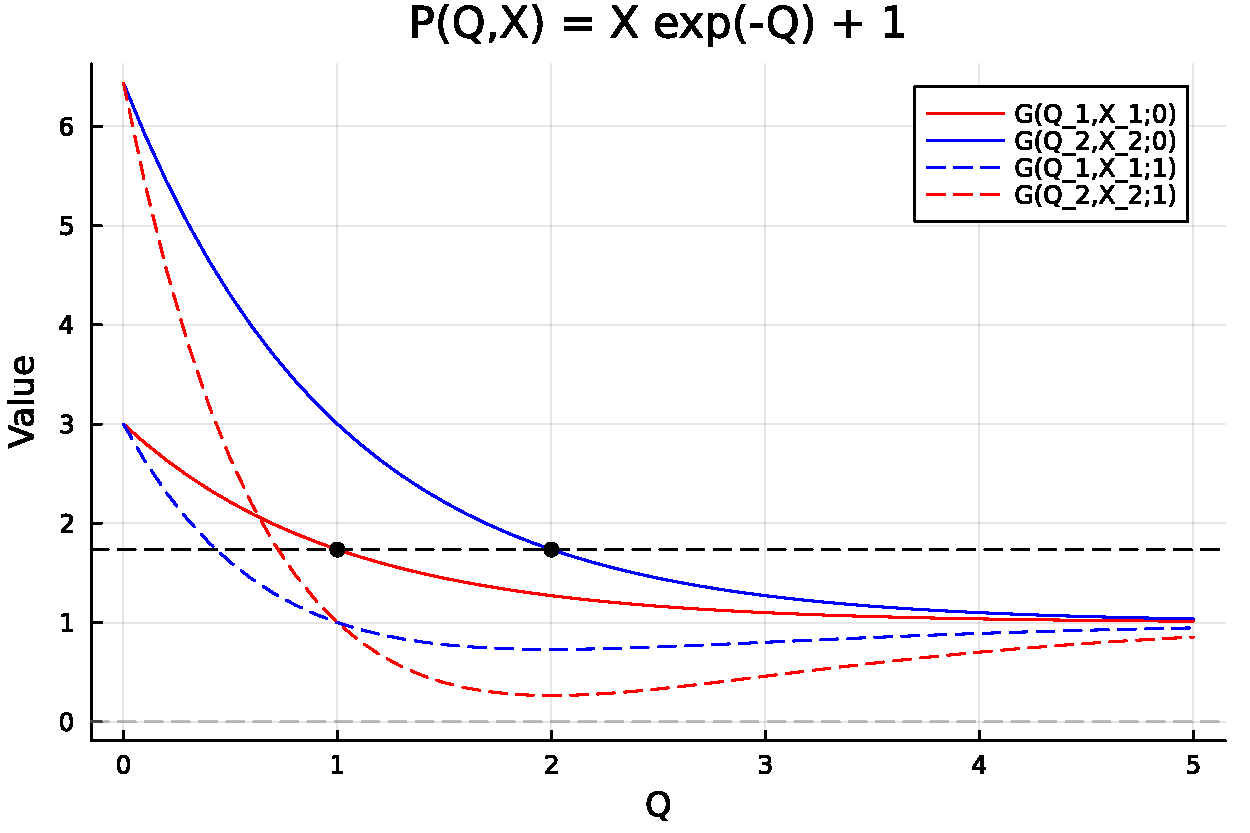
\includegraphics[width=0.8\textwidth]{../figuretable/plot_counter_example.pdf}
\caption{The relationship between $G(Q,X^{d};0)$ and $G(Q,X^{d};1)$}
\label{fig:counterxample_demand_curves}
\end{center}
The graph plots $G(Q,X^{d};0)$ and $G(Q,X^{d};1)$.
The solid lines represent $G(Q,X^{d};0)$ and the dashed lines represent $G(Q,X^{d};1)$.
The color corresponds to $(Q_1, X_1)$ and $(Q_2, X_2)$.
$G(Q,X^{d};0)$ takes the same value, but $G(Q,X^{d};1)$ takes different values under $(Q_1, X_1)$ and $(Q_2, X_2)$.
\end{figure}



At least, based on the assumptions and the argument in Lau's original proof, we cannot guarantee that a separable inverse demand function implies non-identification.
The correct assumption could be "inverse demand functions that guarantee the existence of transformation $T$".
For example $P(Q, X) = Q^{-1/2}X^{d}$ is a separable function and can guarantee the existence because 
\begin{align}
    \frac{\partial P}{\partial Q}(Q, X^{d})Q  = -\frac{1}{2}Q^{-\frac{1}{2}}X^d = \frac{1}{2}P(Q,X^{d}).
\end{align}



\section{Discussion}

\subsection{Relation to the recent literature on distinguishing firm conduct}

The sufficiency of separability implies that if the conduct parameter and marginal cost are simultaneously identified, the demand function is non-separable or satisfies the specific separable function form.
However, the recent literature uses a broader variation in markets for the identification of conduct beyond demand shifters and rotators.
For example, in the differentiated product environment, \citet{berry2014identification} demonstrate that the change in marginal cost or the market size is useful, and hence demand rotation instruments are not necessary to identify conduct.

Of course, homogeneous product settings are more restricted than differentiated product settings.
Even so, Lau's proof of sufficiency does not show that unless a separable demand satisfies  \eqref{eq:identification_separable}, there always exist two distinct pairs of conduct parameter and marginal cost.
Therefore, there could be a separable function except \eqref{eq:identification_separable} that can achieve identification based on other variations in markets.



\newpage
\bibliographystyle{aer}
\bibliography{conduct_parameter}
\appendix

\section{A counterexample}

We show that the conduct parameter is identified when the inverse demand function is separable. 
Consider the following inverse demand function and marginal cost function:
\begin{align}
    P & = \exp(\varepsilon_{d}) Q^{\alpha_0} X_{d1}^{\alpha_1}X_{d2}^{\alpha_2}\label{eq:counter_demand}\\
    MC & = \exp(\varepsilon_{s})Q^{\beta_0} X_{s1}^{\beta_1} X_{s2}^{\beta_2}.\label{eq:counter_mc}
\end{align}
Assume that $\alpha_0 <0$.
The above model does not have an intercept in both the demand function and the marginal cost function. 

The inverse demand function is separable because
\begin{align}
    \frac{\partial }{\partial Q} \left(\frac{\partial P/\partial X_{d1}}{\partial P/\partial X_{d2}} \right) = \frac{\partial }{\partial Q} \left(\frac{\alpha_{1}\exp(\varepsilon_{d}) Q^{-\alpha_0} X_{d1}^{\alpha_1-1}X_{d2}^{\alpha_2}}{\alpha_2\exp(\varepsilon_{d}) Q^{-\alpha_0} X_{d1}^{\alpha_1}X_{d2}^{\alpha_2-1}} \right) =  \frac{\partial }{\partial Q}\left(\frac{\alpha_1}{\alpha_2} \frac{X_{d2}}{X_{d1}} \right)=0.
\end{align}
Thus Theorem \ref{theorem_lau} implies that the conduct parameter cannot be identified.
By taking logarithm to \eqref{eq:counter_demand}, we have a log-linear demand equation such that 
\begin{align}
    \log P = \alpha_0 \log Q + \alpha_1 \log X_{d1}  + \alpha_2 \log X_{d2} + \varepsilon_{d}.\label{eq:counter_demand_equation}
\end{align}
From the first-order condition, 
\begin{align}
    MC = Q^{\beta_0} X_{s1}^{\beta_1}X_{s2}^{\beta_2}\exp(\varepsilon_{s}) & = P + \theta (\alpha_0 \exp(\varepsilon_{d})Q^{\alpha_0-1}X_{d1}^{\alpha_1}X_{d2}^{\alpha_2}) Q\\
    & = P + \theta \alpha_0 P\\
    &= (1 + \theta\alpha_0) P.
\end{align}
By taking a logarithm, we obtain a log-linear supply equation,
\begin{align}
    \log P = - \log(1 + \theta\alpha_0) + \beta_0 \log Q + \beta_1 \log X_{s1}+\beta_2 \log X_{s2} + \varepsilon_{s}.\label{eq:counter_supply_equation}
\end{align}
By solving \eqref{eq:counter_demand_equation} and \eqref{eq:counter_supply_equation}, the equilibrium quantity $Q$ is obtained as
\begin{align}
    \log Q = \frac{\beta_1 \log X_{s1}+\beta_2 \log X_{s2} - \log(1 + \theta\alpha_0)+ \varepsilon_{s} - \alpha_1 \log X_{d1}  - \alpha_2 \log X_{d2} - \varepsilon_{d} }{\alpha_0 - \beta_0}.
\end{align}

Note that the demand parameters can be identified when $X^s$ is a vector of exclusive demand instruments.
Thus we can assume that $\alpha_0, \alpha_1$, and $\alpha_2$ is known.  

Then it is easy to see that $- \log(1 + \theta\alpha_0), \beta_0$, and $\beta_1$ are identified with a vector of exclusive supply instrument $X^d$.
Let $\gamma = - \log(1 + \theta\alpha_0)$, then $\theta = (\exp(-\gamma) - 1)/\alpha_0$.
Because $\alpha_0$ is identified, the parameter $\theta$ is also identified, which contradicts Theorem \ref{theorem_lau}.
\begin{remark}
    The above inverse demand function has a constant-elasticity property. 
    Note that $\alpha_0 \ne \frac{1}{\theta}$ holds.
    Thus it is not the separable function that allows identification in Theorem \ref{theorem_lau}.
    However, \citet{lau1982identifying} states that under this functional form, the conduct parameter cannot be identified in his comment (2) in p 98.
\end{remark}

\begin{remark}
    When the demand equation and the marginal cost equation have an intercept, the identification is impossible because the constant term in \eqref{eq:counter_supply_equation} becomes $-\log(1+\theta \alpha_0) + \beta$ and $\beta$ and $\theta$ cannot be separately identified without additional variables such as demand rotation parameter.
\end{remark}



\section{Interpretation}


Let's return to the original idea in \citet{bresnahan1982oligopoly}.
He essentially considers the following model:
\begin{align}
    P & = \alpha_0 - \alpha_1 Q + \alpha_2 Y + \varepsilon_d,\label{eq:bresnahan_demand} \\
    MC & = \beta_0 + \beta_1 Q + \beta_2 W + \varepsilon_s. \label{eq:bresnahan_marginal_cost}
\end{align}
Assume that $\alpha_1>0$ and $\beta_1 >0$.
The total revenue is 
\begin{align}
    TR(Q) = PQ = \alpha_0Q - \alpha_1 Q^2 + \alpha_2 YQ + \varepsilon_d Q,
\end{align}
and hence, the marginal revenue becomes
\begin{align}
    MR = \alpha_0 - 2\alpha_1 Q + \alpha_2 Y + \varepsilon_d. \label{eq:bresnahan_marginal_revenue}
\end{align}
Note that the slope of the marginal revenue is twice as steep as the demand function under a linear demand model.
Based on the first-order condition, the supply relation can be computed as
\begin{align}
    P & = \beta_0 + (\beta_1 + \theta\alpha_1) Q  + \beta_2 W + \varepsilon_s.\label{eq:bresnahan_supply}
\end{align}
The intersection of \eqref{eq:bresnahan_demand} and \eqref{eq:bresnahan_supply} derives the equilibrium price and the equilibrium quantity.
For example, let's consider perfect competition ($\theta = 0$) and monopoly ($\theta = 1$).
When $\theta = 0$, \eqref{eq:bresnahan_supply} implies that $P = MC$, and the equilibrium quantity under perfect competition is
\begin{align}
    Q^C = \frac{\alpha_0 + \alpha_2 Y - \beta_0 - \beta_2 W+ \varepsilon_d - \varepsilon_s}{\alpha_1 + \beta_1}
\end{align}
In contrast, the monopoly implies that $P = MR$, and the equilibrium quantity under monopoly is
\begin{align}
    Q^m = \frac{\alpha_0 + \alpha_2 Y - \beta_0 - \beta_2 W+ \varepsilon_d - \varepsilon_s}{2\alpha_1 + \beta_1}.
\end{align}

Let $(\beta_0^c, \beta_1^c, \beta_2^c)$ be the parameters of the marginal cost rationalizing the perfect competition and $(\beta_0^m, \beta_1^m, \beta_2^m)$ be that rationalizing monopoly. 
For example, suppose that $\beta_1^c = \alpha_1 + \beta_1^m$.
The monopoly cost is flatter than the perfect competition cost.
In this case, the equilibrium quantity is the same in both models ($Q^c = Q^m$) because the denominator has the same value, and hence, the researcher cannot distinguish two models from the data.

Figure \ref{fig:bresnahan_non_identification} illustrates this situation.
Let $MC^c$ be the marginal cost rationalized by the perfect competition and $MC^m$ be the marginal cost rationalized by the monopoly.
$E_1$ is the observed equilibrium outcome, and both models rationalize the equilibrium.
Furthermore, the demand shift due to the increase of $Y$ does not help identify the conduct, which equally increases $Q^c$ and $Q^m$, and $E_2$, the new equilibrium point, is still rationalized by both models.

We can also demonstrate that the conduct parameter cannot be identified from the supply relation.
Let $\gamma = (\beta_1 + \theta \alpha_1)$.
Then, the parameter can be identified  in \eqref{eq:bresnahan_supply}are $\beta_0$,$\gamma$, and $\beta_2$, but we cannot identify $\theta$ as $\gamma$ in both models has the same value: 
\begin{align}
    \gamma^c &= \beta_1^c + \theta \alpha_1 = \beta^c = \beta_1^m + \alpha_1 = \gamma^m.
\end{align}

\begin{figure}
    \begin{center}
        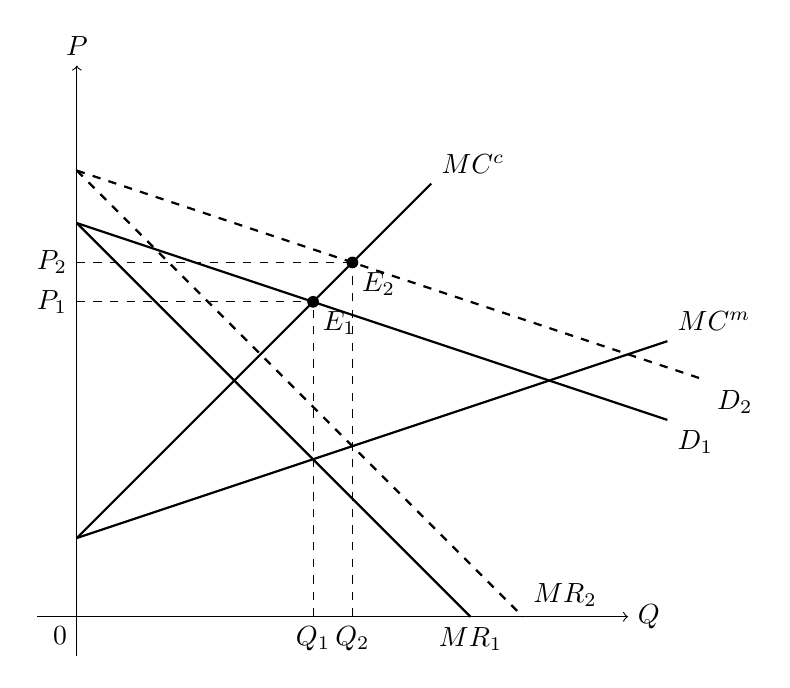
\begin{tikzpicture}
        % Axes
        \draw[->] (-0.5,0) -- (7,0) node[right] {$Q$}; % Horizontal axis
        \draw[->] (0,-0.5) -- (0,7) node[above] {$P$}; % Vertical axis
    
        % Demand Curve (D_1) - passes through (0,5), (3,4), and (7.5,2.5)
        \draw[thick] (0,5) -- (7.5,2.5) node[below right] {$D_1$};
    
        % Marginal Revenue (MR_1) - passes through (0,5), (3,2), and (5,0)
        \draw[thick] (0,5) -- (5,0) node[below] {$MR_1$};
    
        % Supply Curve under competition (S^c) - passes through (0,1), (3,4), and (4.5,5.5)
        \draw[thick] (0,1) -- (4.5,5.5) node[above right] {$MC^c$};
    
        % Supply Curve under monopoly (S^m) - passes through (0,1), (3,2), and (7.5,3.5)
        \draw[thick] (0,1) -- (7.5,3.5) node[above right] {$MC^m$};
    
        % Equilibrium point (E_1) - intersection of D_1 and S^c at (3,4)
        \node[circle, fill, inner sep=1.5pt] (E1) at (3,4) {};
        \node[below right] at (E1) {$E_1$};
    
    
        % Equilibrium point (E_2) - intersection of D_1 and S^c at (7/2,9/2)
        \node[circle, fill, inner sep=1.5pt] (E2) at (7/2,9/2) {};
        \node[below right] at (E2) {$E_2$};
    
        % Shifted Demand Curve (D_1 shifted)
        \draw[thick, dashed] (0,34/6) -- (8,3) node[below right] {$D_2$};
        
        % Shifted MR (MR_1 shifted)
        \draw[thick, dashed] (0,34/6) -- (34/6,0) node[above right] {$MR_2$};
        
        % Dashed lines for price and quantity
        \draw[dashed] (3,0) -- (3,4);
        \draw[dashed] (0,4) -- (3,4);
    
        \draw[dashed] (0,9/2) -- (7/2,9/2);
        \draw[dashed] (7/2,0) -- (7/2,9/2);
    
        % Additional labels
        \node[below left] at (0,0) {0};
        \node[left] at (0,4) {$P_1$};
        \node[below] at (3,0) {$Q_1$};
    
        \node[left] at (0,9/2) {$P_2$};
        \node[below] at (7/2,0) {$Q_2$};
    \end{tikzpicture}
    \end{center}
    \caption{The illustration of the non-identification result}
    \label{fig:bresnahan_non_identification}
    \vspace{2mm}
    \footnotesize
    Note: $MC^c$ is the marginal cost rationalized by the perfect competition, and $MC^m$ is the marginal cost rationalized by the perfect competition. $\beta_c = \beta_m + \alpha_1$ holds.
    The perfect competition and the monopoly rationalize the equilibrium point $E_1$. The shift in the demand does not help because the new equilibrium $E_2$ still are rationalized by both models.
\end{figure}


Let's consider our case.
The simplified version of our example is the following:
\begin{align}
    P & = \exp(\varepsilon_{d}) Q^{-\alpha_0} Y^{\alpha_1},\label{eq:simple_demand} \\
    MC & = \exp(\varepsilon_{s}) Q^{\beta_0} W^{\beta_1}. \label{eq:simple_marginal_cost}
\end{align}
The total revenue is
\begin{align}
    TR = PQ = \exp(\varepsilon_{d}) Q^{-\alpha_0+1} Y^{\alpha_1},
\end{align}
and hence, the marginal revenue is
\begin{align}
    MR = (-\alpha_0+1)\exp(\varepsilon_{d}) Q^{-\alpha_0} Y^{\alpha_1}
\end{align}
Take the logarithm of the demand and the marginal revenue, we have
\begin{align}
    \log P & = -\alpha_0 \log Q + \alpha_1 \log Y + \varepsilon_d,\\
    \log MR& = \log (1 -\alpha_0) -\alpha_0 \log Q + \alpha_1 \log Y + \varepsilon_d.
\end{align}
On the other hand, the supply relation becomes
\begin{align}
    \log P = -\log (1 - \theta \alpha_0) + \beta_0 \log Q + \beta_1 \log W + \varepsilon_s. \label{eq:simple_supply}
\end{align}

While the conduct parameter changes the slope of the supply relation in Bresnahan's example, the change in the conduct parameter shifts the supply relation in our example.
To make the model feasible, we assume that $1- \theta \alpha_0 >0$ for any $\theta \in [0,1]$.
Because $\alpha_0>0$ and $\theta \in [0,1]$, $1- \theta\alpha_0 <1$, which implies that $- \log(1- \theta\alpha_0) > 0$.
Then, for example, when we compare perfect competition and monopoly,  the supply relations under perfect competition and monopoly are parallel by $\log(1 - \alpha_0)$, and the supply relation under monopoly is shifted upward to the supply relation under perfect competition.

Note also that $\log (1 - \alpha_0)$ parallels the demand function and the marginal revenue, and the marginal revenue is shifted downwards.

Figure \ref{fig:simpe_identification} plots the above equations as in Bresnahan's example.
As we can see, under perfect competition and monopoly, the equilibrium quantities under the two models differ.

and the equilibrium quantity is given by
\begin{align}
    \log Q_t &= \frac{ \log (1 - \theta \alpha_0 ) + \alpha_1 \log Y_t - \beta_2 \log W_{t} + \varepsilon^{d} - \varepsilon^{c}}{\alpha_0 + \beta_0 }.\label{eq:quantity_loglinear}
\end{align}

\begin{figure}[t]
    \centering
        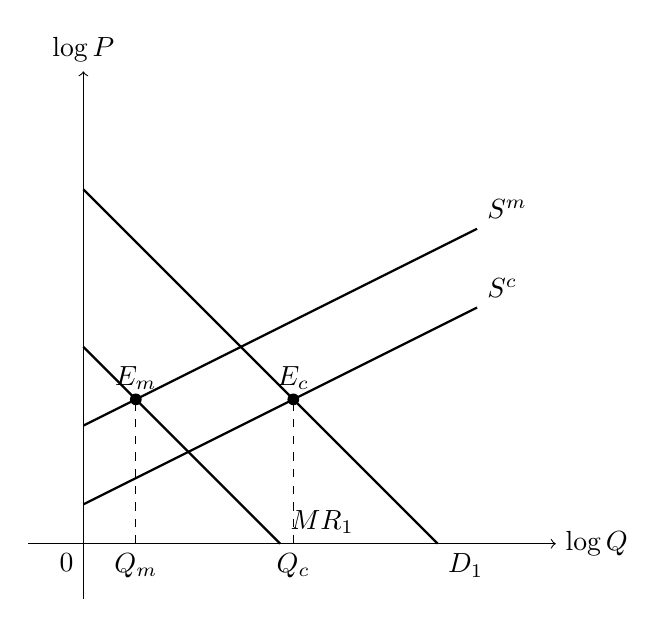
\begin{tikzpicture}
            % Axes
            \draw[->] (-0.7,0) -- (6,0) node[right] {$\log Q$}; % Horizontal axis
            \draw[->] (0,-0.7) -- (0,6) node[above] {$\log P$}; % Vertical axis

            % Marginal Revenue (MR_1) - passes through (0,5), (3,2), and (5,0)
            \draw[thick] (0,4.5) -- (4.5,0) node[below right] {$D_1$};
            \draw[thick] (0,2.5) -- (2.5,0) node[above right] {$MR_1$};
            
            % Supply Curve under competition (S^c) - passes through (0,1), (3,4), and (4.5,5.5)
            \draw[thick] (0,1.5) -- (5,4) node[above right] {$S^m$};
            % Supply Curve under monopoly (S^m) - passes through (0,1), (3,2), and (7.5,3.5)
            \draw[thick] (0,0.5) -- (5,3) node[above right] {$S^c$};

            % Equilibrium point (E_1) - intersection of D_1 and S^c at (3,4)
            \node[circle, fill, inner sep=1.5pt] (Ec) at (2/3,11/6) {};
            \node[above] at (Ec) {$E_m$};

            \node[circle, fill, inner sep=1.5pt] (Em) at (8/3,11/6) {};
            \node[above] at (Em) {$E_c$};
            % Additional labels
            \node[below left] at (0,0) {0};
            \node[below] at (2/3, 0) {$Q_m$};
            \node[below] at (8/3, 0) {$Q_c$};

            \draw[dashed] (8/3,0) -- (8/3,11/6);
            \draw[dashed] (2/3,0) -- (2/3,11/6);
        \end{tikzpicture}
        \caption{}
    \caption{Identification of the conduct under the log-linear model}
    \label{fig:simpe_identification}
\end{figure}



\end{document}